\section{Motivation}
The motivation for the project stems from the lack of a simple enough tool to demonstrate the dynamics of an evolving population. While multiple systems implementing genetic algorithms are available, they tend to be obsolete, no longer supported, or generally intended as frameworks providing only the algorithms to be used in optimization. The project is intended as a light-weight educational tool, in order to provide insight into the basic function of genetic algorithms, together with presenting the dynamics of an evolving population.

\section{Background}
There has been significant research in the field of Genetic Algorithms. When faced with complex optimization problems, performing a linear search, especially through a large solution space usually associated with such problems, may prove ineffective. 

While initially proposed by Alan Turing in 1950, evolutionary algorithms became regarded as a method of solving complex optimisation problems in the 1970s. In general, several biological methods (such as sexual or asexual reproduction or genetic mutation) are used in order to evolve the population of a particular system with respect to a certain predetermined fitness function. As such, more "fit" individuals have a higher chance of being selected to pass on their genome to the next generation, thus increasing the fitness factor of the overall population after each iteration. Over a longer period of time (spanning from a few thousand, to a million generations), the population will evolve towards a solution. This, however, suffers from diminishing returns, as the population tends to meet an impasse in locally optimal points, rather than reach the global maximum.

(add section in which terms are defined)

\subsection{Previous Work}
A more prominent paper in the field of artificial evolution is "Evolving Virtual Creatures" by Karl Sims \cite{sims1994evolving}. The paper details an evolutionary system which focuses evolving a population of creatures consisting of three dimensional blocks with respect to various movement-specific tasks (such as walking, running, jumping, climbing, and swimming). Noteworthy is the fact that both the creature's morphology and it's "brain" are evolved. While the initial randomly created generation was incapable of performing any task, subsequent generations, showed significant improvement. Even after a relatively low number of generations, some creatures were becoming adapted to their environment. In the swimming example, some creatures were successful in developing fin-like appendages, used for locomotion, while other replicated the waving motion of water-snakes. The scope of the experiment, however is quite limited, as creatures are observed individually, with a rather basic fitness function, and not in competition with each other.

A more recent paper \cite{lessin2013open} deals with the open-ended nature of evolution, previously unexplored in Karl Sims's paper. The paper proposes the evolution a creature's brains as well as body, thus allowing it to better adapt to its environment. While the evolution of the body is fairly similar to the method described by Karl Sims, the control part of a creature is evolved differently. This involves encapsulation a creature's previously learned skills. The benefits presented are persistent memory, allowing a creature to store a certain behaviour once it has been learned, and overall simplicity, allowing the whole procedure to be called as a single node, instead of actively recreating the movement. By allowing newer nodes to be modified more frequently than older ones, the algorithm simulates the forming of habits. By changing the fitness function, creatures can adapt to different environments, or learn more complex behaviours, without "forgetting" their previous training. This, in turn, provides a more accurate representation of nature.

\subsection{Existing Applications}
While research in the field of Genetic Algorithms is extensive, it deals mostly either with problems of optimization, or with the best few individuals of a population. This is not the case when trying to simulate the entire population, as being the very best only gives a marginally higher chance of passing genes to the next generation. Simply being "good enough" to sufficient food in order to be able to live and reproduce is sufficient.

A similar application is appearance is Darwinbots  (how to cite a wiki?). Darwinbtos presents itself as an artificial life simulator, where creatures, called "bots" can compete for food in a simulated two dimensional environment. The most successful "bots" will live on to pass their genes to subsequent generations.
\begin{figure}[!th]
	\centering
	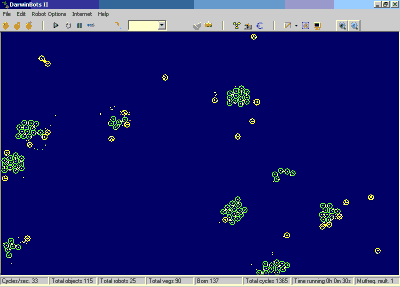
\includegraphics[scale=1]{images/darwinbots}
	\caption{A screenshots from a Darwinbots simulation}
\end{figure}
Darwinbots, however, specialises in simulating Von Neumann probes.

(write more about Darwinbots)

(write about Goopies)

(add section about Conway's game of life / cellular automata)

\section{Overview}
The system simulates a population of individuals, named "blobs", whose sole purpose is reproduction. This is done asexually, when each individual reaches a high enough energy threshold, encoded in his genome. Energy can be gained by eating the food pellets scattered randomly around the world. The "blobs" eat food by colliding with it, and find it by performing a random walk, in this case, a simplified version of a L\'evy walk.
The system is made with interactivity in mind, allowing the user to tweak various parameters of the environment, while observing the population evolves in order to adapt to the change. A user could interact more directly with the simulation by adding "blobs" or placing food. A sudden influx in either will generate a period of instability in the population which eventually reverts back to a stable state.
Information about the population is presented via a graph, showing total number, and average characteristics of the individuals. More specific information about a "blob" in particular is displayed via a pop-up message, should a creature be clicked on.

\section{Dissertation Outline}
The rest of the dissertation presents in detail the process of development of the evolutionary system, comically named "Blobs on a Plane". The outline is as follows:

Chapter 2 details the functional and non-functional requirements, as well as the requirements gathering process.

Chapter 3 discusses various concerns about the design of the system and the user interface, any assumptions, and the design decisions made. Presented are also the initial design ideas and the final design.

Chapter 4 describes the implementation details, choice of framework, some of the evolutionary algorithms used, as well as the project deployment.

Chapter 5 deals primarily with evaluation, from both users and experts, as well as internal testing.

Chapter 6 provides a summary of the project, project management matters, and future work.